\chapter{Array Implementation} % Write in your own chapter title
\label{Chapter4}
\lhead{Chapter 4. \emph{Array Implementation}} % Write in your own chapter title to set the page header

\begin{figure}[H]
	\centering
	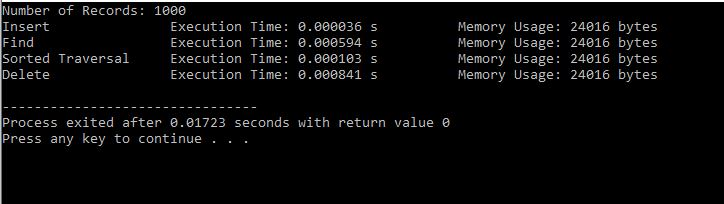
\includegraphics[scale =0.7]{./Figures/Array1000.jpg}
	\rule{35em}{0.5pt}
	\caption{Results for array implementation with data size 1000.}
	\label{fig:Array 1000}
\end{figure}

\begin{figure}[H]
	\centering
	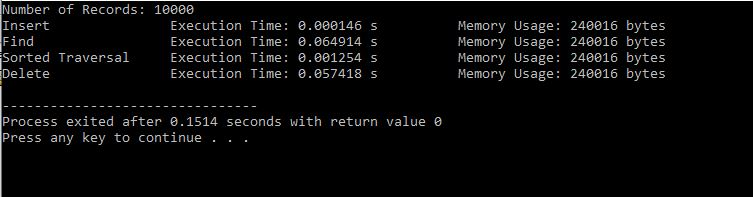
\includegraphics[scale =0.7]{./Figures/Array10000.jpg}
	\rule{35em}{0.5pt}
	\caption{Results for array implementation with data size 10000.}
	\label{fig:Array 10000}
\end{figure}

\begin{figure}[H]
	\centering
	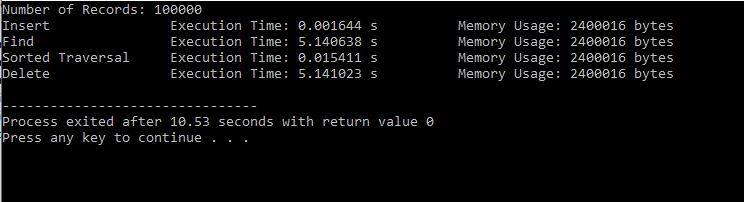
\includegraphics[scale =0.7]{./Figures/Array100000.jpg}
	\rule{35em}{0.5pt}
	\caption{Results for array implementation with data size 100000.}
	\label{fig:Array 100000}
\end{figure}

\begin{figure}[H]
	\centering
	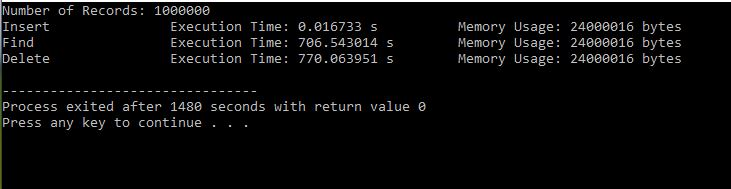
\includegraphics[scale =0.7]{./Figures/Array1000000.jpg}
	\rule{35em}{0.5pt}
	\caption{Results for array implementation with data size 1000000.}
	\label{fig:Array 1000000}
\end{figure}
